\documentclass[a4paper,11pt,draft]{article}

\usepackage[finnish]{babel}
\usepackage[utf8]{inputenc}
\usepackage[margin=1in]{geometry}
\usepackage{amsfonts,amsmath,amssymb,amsthm,enumitem}
\usepackage{pgf}
\usepackage{tikz}
\usetikzlibrary{arrows,automata}

\newtheorem*{claim}{Väite}

\begin{document}

\subsection*{582206 Laskennan mallit, syksy 2012\\
2. Harjoitusten malliratkaisut}

\begin{enumerate}
\item
  Olkoon kahden äärellisen automaatin $M_1$ ja $M_2$ tilat ja
  siirtymät seuraavat.
  
  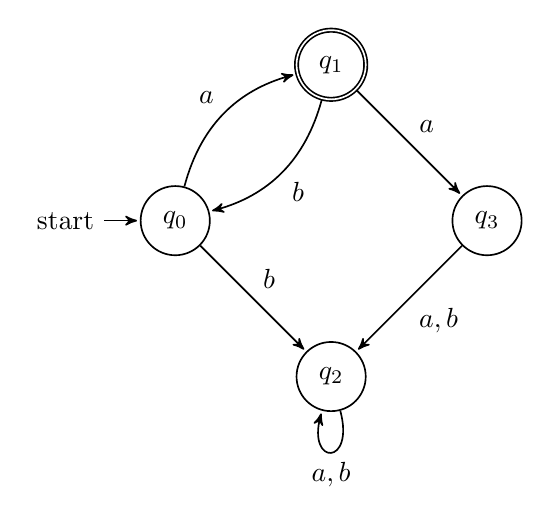
\begin{tikzpicture}[->,>=stealth',shorten >=1pt,auto,node distance=2.8cm,semithick]
    \node[initial,state]   (A)                    {$q_0$};
    \node[accepting,state] (B) [above right of=A] {$q_1$};
    \node[state]           (C) [below right of=A] {$q_2$};
    \node[state]           (D) [below right of=B] {$q_3$};

    \path (A) edge [bend left]  node {$a$} (B)
              edge              node {$b$} (C)
          (B) edge              node {$a$} (D)
              edge [bend left]  node {$b$} (A)
          (C) edge [loop below] node {$a,b$} (C)
          (D) edge              node {$a,b$} (C);
  \end{tikzpicture}

  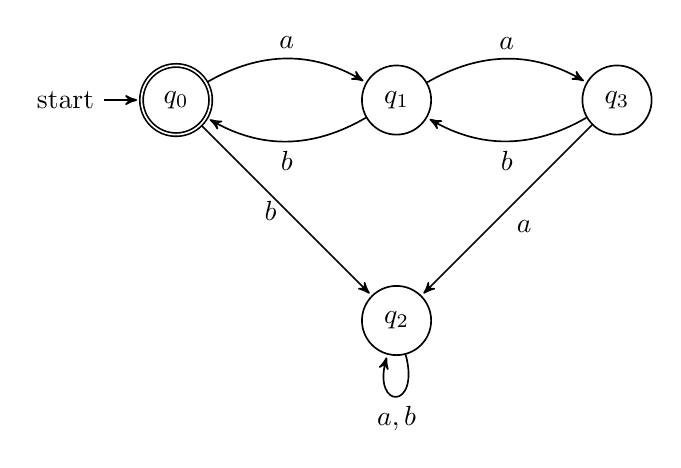
\begin{tikzpicture}[->,>=stealth',shorten >=1pt,auto,node distance=2.8cm,semithick]
    \node[initial,accepting,state]   (A)              {$q_0$};
    \node[state]                     (B) [right of=A] {$q_1$};
    \node[state]                     (C) [below of=B] {$q_2$};
    \node[state]                     (D) [right of=B] {$q_3$};

    \path (A) edge [bend left]   node {$a$}   (B)
              edge               node [left] {$b$}   (C)
          (B) edge [bend left]   node {$a$}   (D)
              edge [bend left]   node {$b$}   (A)
          (C) edge [loop below]  node {$a,b$} (C)
          (D) edge               node {$a$}   (C)
              edge [bend left]   node {$b$}   (B);
  \end{tikzpicture}

  \begin{enumerate}
  \item
    Mikä on kunkin automaatin aloitustila?
  \item
    Mitkä ovat hyväksyviä tiloja?
  \item
    Minkä tilajonon automaatit käyvät läpi syötteellä $aabb$?
  \item
    Hyväksyvätkö automaatit syötteen $aabb$?
  \item
    Hyväksyvätkö automaatit merkkijonon $\varepsilon$?
  \end{enumerate}
\end{enumerate}

\end{document}
